\documentclass[letterpaper,12pt]{article}\usepackage[]{graphicx}\usepackage[]{color}
%% maxwidth is the original width if it is less than linewidth
%% otherwise use linewidth (to make sure the graphics do not exceed the margin)
\makeatletter
\def\maxwidth{ %
  \ifdim\Gin@nat@width>\linewidth
    \linewidth
  \else
    \Gin@nat@width
  \fi
}
\makeatother

\definecolor{fgcolor}{rgb}{0.345, 0.345, 0.345}
\newcommand{\hlnum}[1]{\textcolor[rgb]{0.686,0.059,0.569}{#1}}%
\newcommand{\hlstr}[1]{\textcolor[rgb]{0.192,0.494,0.8}{#1}}%
\newcommand{\hlcom}[1]{\textcolor[rgb]{0.678,0.584,0.686}{\textit{#1}}}%
\newcommand{\hlopt}[1]{\textcolor[rgb]{0,0,0}{#1}}%
\newcommand{\hlstd}[1]{\textcolor[rgb]{0.345,0.345,0.345}{#1}}%
\newcommand{\hlkwa}[1]{\textcolor[rgb]{0.161,0.373,0.58}{\textbf{#1}}}%
\newcommand{\hlkwb}[1]{\textcolor[rgb]{0.69,0.353,0.396}{#1}}%
\newcommand{\hlkwc}[1]{\textcolor[rgb]{0.333,0.667,0.333}{#1}}%
\newcommand{\hlkwd}[1]{\textcolor[rgb]{0.737,0.353,0.396}{\textbf{#1}}}%

\usepackage{framed}
\makeatletter
\newenvironment{kframe}{%
 \def\at@end@of@kframe{}%
 \ifinner\ifhmode%
  \def\at@end@of@kframe{\end{minipage}}%
  \begin{minipage}{\columnwidth}%
 \fi\fi%
 \def\FrameCommand##1{\hskip\@totalleftmargin \hskip-\fboxsep
 \colorbox{shadecolor}{##1}\hskip-\fboxsep
     % There is no \\@totalrightmargin, so:
     \hskip-\linewidth \hskip-\@totalleftmargin \hskip\columnwidth}%
 \MakeFramed {\advance\hsize-\width
   \@totalleftmargin\z@ \linewidth\hsize
   \@setminipage}}%
 {\par\unskip\endMakeFramed%
 \at@end@of@kframe}
\makeatother

\definecolor{shadecolor}{rgb}{.97, .97, .97}
\definecolor{messagecolor}{rgb}{0, 0, 0}
\definecolor{warningcolor}{rgb}{1, 0, 1}
\definecolor{errorcolor}{rgb}{1, 0, 0}
\newenvironment{knitrout}{}{} % an empty environment to be redefined in TeX

\usepackage{alltt}
\usepackage[top=1in,bottom=1in,left=1in,right=1in]{geometry}
\usepackage{setspace}
\usepackage[colorlinks=true,urlcolor=blue,citecolor=blue,linkcolor=blue]{hyperref}
\usepackage{indentfirst}
\usepackage{multirow}
\usepackage{booktabs}
\usepackage[final]{animate}
\usepackage{graphicx}
\usepackage{verbatim}
\usepackage{rotating}
\usepackage{tabularx}
\usepackage{array}
\usepackage{subfig} 
\usepackage[noae]{Sweave}
\usepackage{cleveref}
\usepackage[figureposition=bottom]{caption}
\usepackage{paralist}
\usepackage{acronym}
\usepackage{outlines}
\usepackage{pdflscape}

% knitr options




\IfFileExists{upquote.sty}{\usepackage{upquote}}{}
\begin{document}

\begin{landscape}
\centering\vspace*{\fill}
\begin{figure}[!ht]

{\centering 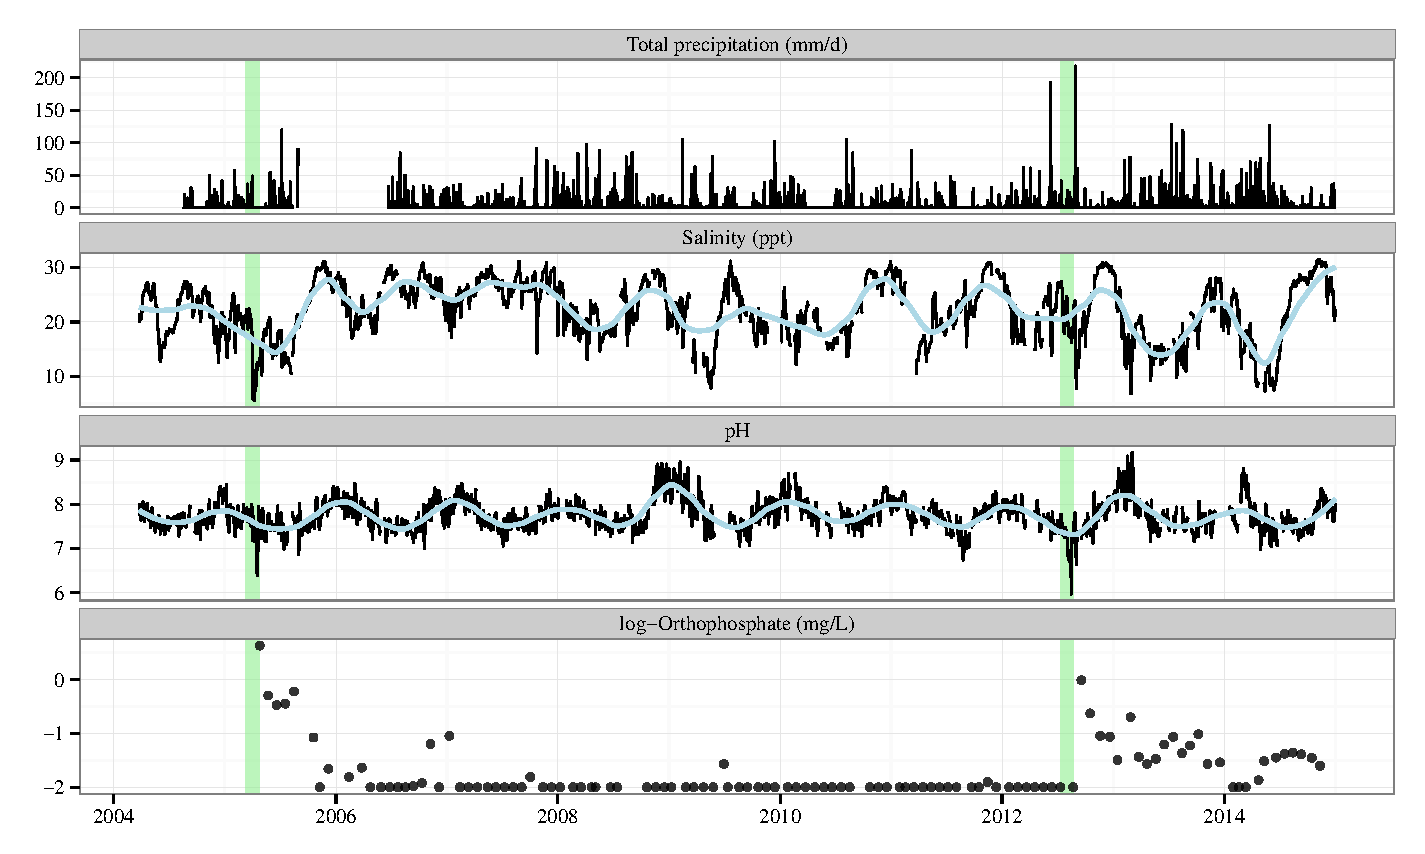
\includegraphics[width=\maxwidth,height=5in]{figs/tsplot-1} 

}

\caption[Time series of total precipitation, salinity, pH, and phosphate for Bangs Lake, Grand Bay reserve]{Time series of total precipitation, salinity, pH, and phosphate for Bangs Lake, Grand Bay reserve.  Vertical green bars indicate a heavy rain event in April 2005 and hurricane Isaac in August 2012.  Salinity and pH include a loess smooth to reduce variability. Orthophosphate is colored by event categories in relation to the vertical green bars.  E1A: event 1 acute, E1C: event 1 chronic, NI: non-impact, E2A: event 2 acute, E2C: event 2 chronic.}\label{fig:tsplot}
\end{figure}


\end{landscape}
\clearpage

\begin{figure}[!ht]

{\centering 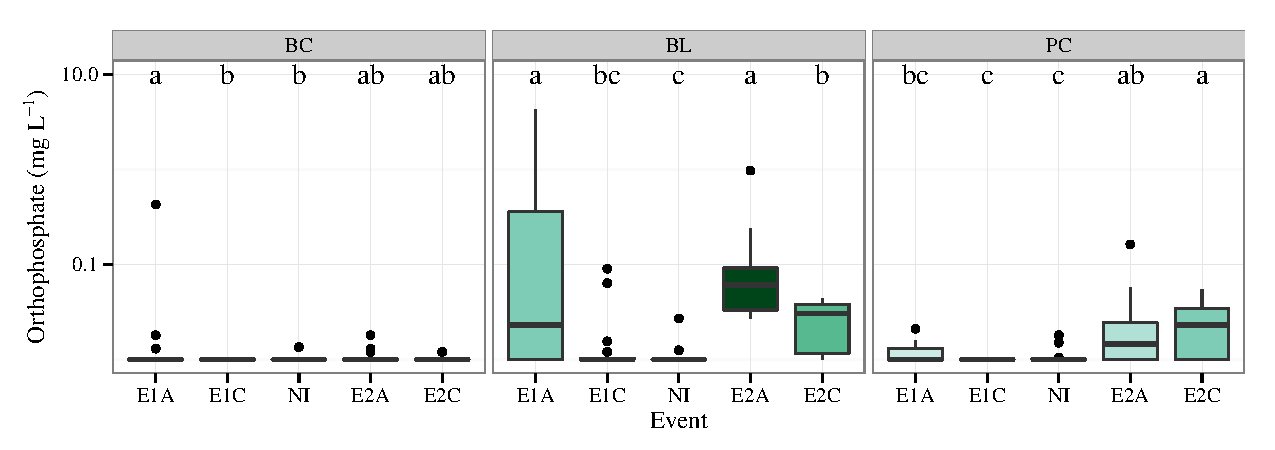
\includegraphics[width=\maxwidth]{figs/tukey-1} 

}

\caption[Boxplot summaries by event of monthly orthophosphate data at Bayou Cumbest (BC), Bangs Lake (BL), and Point aux Chenes (PC) sites in Grand Bay]{Boxplot summaries by event of monthly orthophosphate data at Bayou Cumbest (BC), Bangs Lake (BL), and Point aux Chenes (PC) sites in Grand Bay.  Letters indicate events with significantly different events based on Tukey multiple comparison analysis within each site.  Boxes represent the interquartile range (IQR, 25\textsuperscript{th} to 75\textsuperscript{th} percentile) with the median as the middle horizonal line.  Outliers are present beyond whiskers (1.5$\cdot$IQR). Boxes are shaded by medians between sites.  E1A: event 1 acute, E1C: event 1 chronic, NI: non-impact, E2A: event 2 acute, E2C: event 2 chronic.}\label{fig:tukey}
\end{figure}


\clearpage

\begin{figure}[!ht]

{\centering 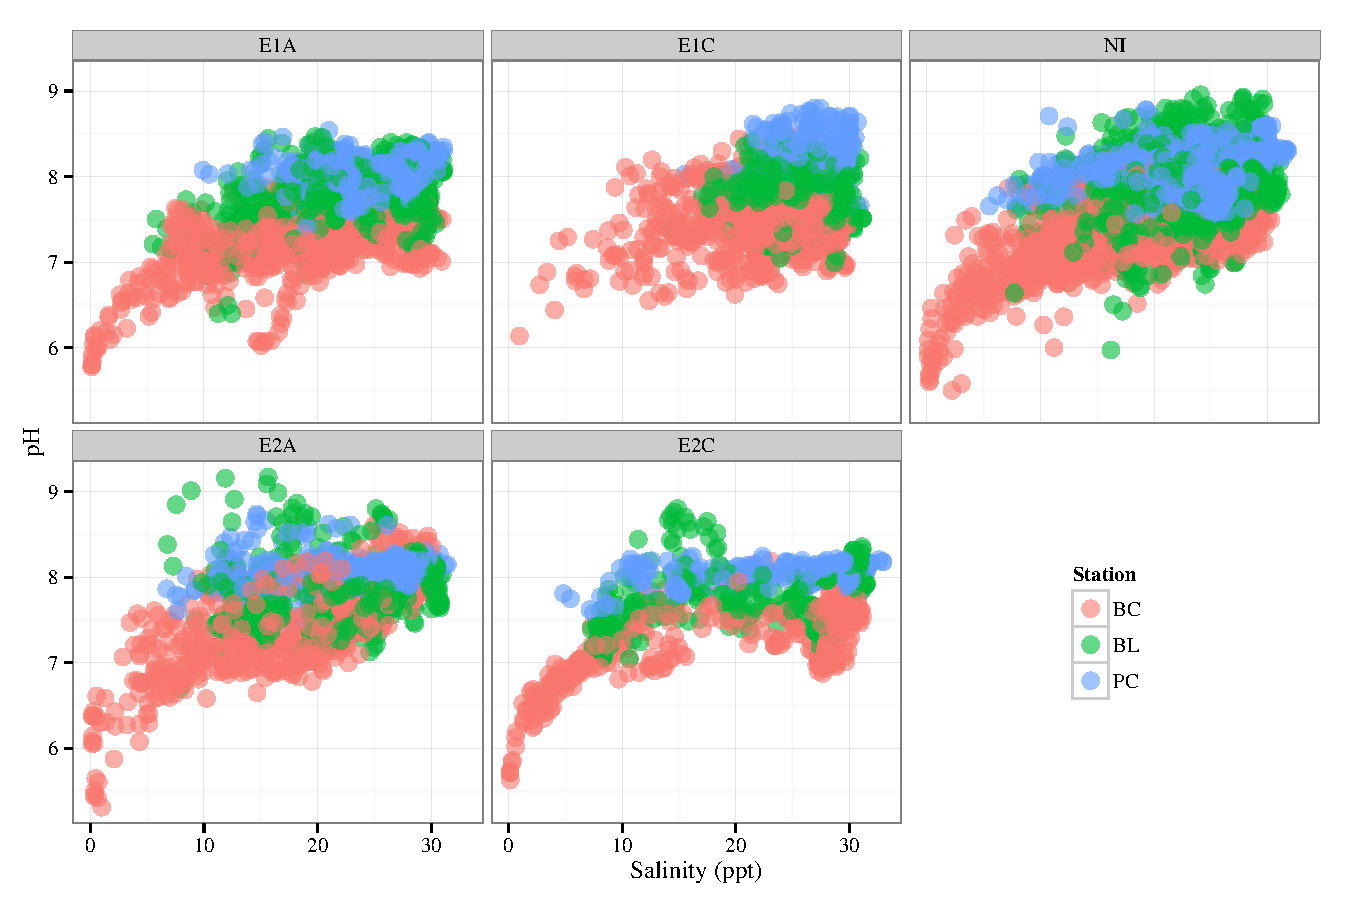
\includegraphics[width=\maxwidth]{figs/phvsal1-1} 

}

\caption[Scatterplots of pH versus salinity for each of the time frames, grouped by station]{Scatterplots of pH versus salinity for each of the time frames, grouped by station.  Observations are daily averages from the continuous time series. E1A: event 1 acute, E1C: event 1 chronic, NI: non-impact, E2A: event 2 acute, E2C: event 2 chronic.}\label{fig:phvsal1}
\end{figure}


\clearpage

\begin{figure}[!ht]

{\centering 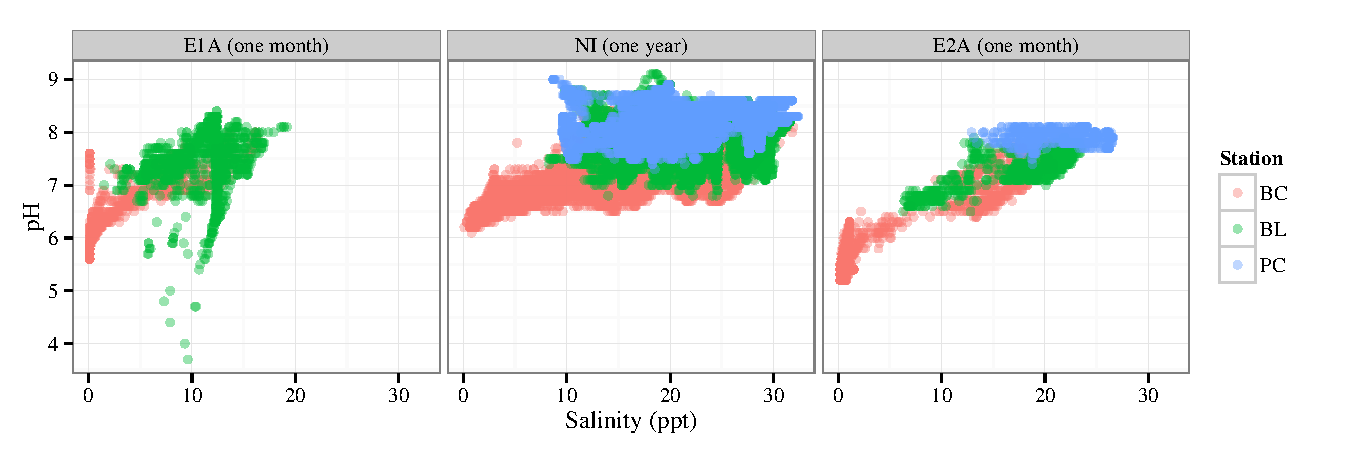
\includegraphics[width=\maxwidth]{figs/phvsal2-1} 

}

\caption[Scatterplots of pH versus salinity for one month following the two acute exposure events (E1A, E2A) and 2010 during the non-impact (NI) time frame]{Scatterplots of pH versus salinity for one month following the two acute exposure events (E1A, E2A) and 2010 during the non-impact (NI) time frame.  Values are thirty-minute observations at each station. E1A: event 1 acute, NI: non-impact, E2A: event 2 acute.}\label{fig:phvsal2}
\end{figure}


\clearpage

%latex.default(totab, file = "", rowlabel = "Site comparisons",     caption = cap.val, caption.loc = "top", rgroup = rgroups,     n.rgroup = rep(3, 2), cgroup = c("First acute event (E1A)",         "Second acute event (E2A)"), n.cgroup = c(2, 2), rowname = wqres$L1,     label = "tab:ccfwq", insert.bottom = foot.val, col.just = c("r",         "c", "r", "c"))%
\begin{table}[!tbp]
\caption{Results of cross-correlation analyses comparing water quality time series between sites at Grand Bay during the two acute event periods.  Values for pH and salinity (ppt) are the lags in the compared time series between sites at which the maximum correlation was observed.  Negative lags indicate observations were leading at the first site relative to the second, whereas positive lags indicate observations lagged at the first site relative to the second.  One lag is thirty minutes.\label{tab:ccfwq}} 
\begin{center}
\begin{tabular}{lrccrc}
\hline\hline
\multicolumn{1}{l}{\bfseries Site comparisons}&\multicolumn{2}{c}{\bfseries First acute event (E1A)}&\multicolumn{1}{c}{\bfseries }&\multicolumn{2}{c}{\bfseries Second acute event (E2A)}\tabularnewline
\cline{2-3} \cline{5-6}
\multicolumn{1}{l}{}&\multicolumn{1}{c}{Lag}&\multicolumn{1}{c}{Correlation}&\multicolumn{1}{c}{}&\multicolumn{1}{c}{Lag}&\multicolumn{1}{c}{Correlation}\tabularnewline
\hline
{\bfseries pH}&&&&&\tabularnewline
~~BC - PC&$ 1$&$0.25$&&$ 1$&$0.40$\tabularnewline
~~BL - BC&$-1$&$0.58$&&$ 0$&$0.54$\tabularnewline
~~BL - PC&$ 0$&$0.57$&&$ 1$&$0.54$\tabularnewline
\hline
{\bfseries Salinity}&&&&&\tabularnewline
~~BC - PC&$ 1$&$0.47$&&$40$&$0.70$\tabularnewline
~~BL - BC&$ 0$&$0.86$&&$ 0$&$0.92$\tabularnewline
~~BL - PC&$ 5$&$0.73$&&$40$&$0.87$\tabularnewline
\hline
\end{tabular}\end{center}

\footnotesize BC: Bayou Cumbest, BL: Bangs Lake, PC: Point aux Chenes\end{table}

\clearpage

%latex.default(totab, file = "", rowlabel = "Site comparisons",     caption = cap.val, caption.loc = "top", rgroup = rgroups,     n.rgroup = rep(3, 4), cgroup = c("First acute event (E1A)",         "Second acute event (E2A)"), n.cgroup = rep(2, 2), rowname = nutres$L1,     label = "tab:ccfnut", insert.bottom = foot.val, col.just = c("r",         "c", "r", "c"))%
\begin{table}[!tbp]
\caption{Results of cross-correlation analyses comparing nutrient time series between sites at Grand Bay during the two acute event periods.  Values are the lags for each nutrient varialbe in the compared time series between sites at which the maximum correlation was observed.  Negative lags indicate observations were leading at the first site relative to the second, whereas positive lags indicate observations lagged at the first site relative to the second.  One lag is one month.\label{tab:ccfnut}} 
\begin{center}
\begin{tabular}{lrccrc}
\hline\hline
\multicolumn{1}{l}{\bfseries Site comparisons}&\multicolumn{2}{c}{\bfseries First acute event (E1A)}&\multicolumn{1}{c}{\bfseries }&\multicolumn{2}{c}{\bfseries Second acute event (E2A)}\tabularnewline
\cline{2-3} \cline{5-6}
\multicolumn{1}{l}{}&\multicolumn{1}{c}{Lag}&\multicolumn{1}{c}{Correlation}&\multicolumn{1}{c}{}&\multicolumn{1}{c}{Lag}&\multicolumn{1}{c}{Correlation}\tabularnewline
\hline
{\bfseries Chlorophyll a}&&&&&\tabularnewline
~~BC - PC&$ 0$&$0.63$&&$-1$&$0.52$\tabularnewline
~~BL - BC&$ 0$&$0.49$&&$ 1$&$0.49$\tabularnewline
~~BL - PC&$ 0$&$0.92$&&$ 0$&$0.87$\tabularnewline
\hline
{\bfseries Ammonium}&&&&&\tabularnewline
~~BC - PC&$ 0$&$0.99$&&$-4$&$0.38$\tabularnewline
~~BL - BC&$ 0$&$0.96$&&$ 2$&$0.57$\tabularnewline
~~BL - PC&$ 0$&$0.89$&&$ 0$&$0.71$\tabularnewline
\hline
{\bfseries Nitrite + Nitrate}&&&&&\tabularnewline
~~BC - PC&$ 0$&$0.70$&&$ 6$&$0.94$\tabularnewline
~~BL - BC&$ 0$&$0.81$&&$ 0$&$0.11$\tabularnewline
~~BL - PC&$-3$&$0.55$&&$-5$&$0.98$\tabularnewline
\hline
{\bfseries Orthophosphate}&&&&&\tabularnewline
~~BC - PC&$-6$&$0.60$&&$ 1$&$0.78$\tabularnewline
~~BL - BC&$ 0$&$0.62$&&$-1$&$0.79$\tabularnewline
~~BL - PC&$-6$&$0.49$&&$ 0$&$0.82$\tabularnewline
\hline
\end{tabular}\end{center}

\footnotesize BC: Bayou Cumbest, BL: Bangs Lake, PC: Point aux Chenes\end{table}

\clearpage

% appendix boxplots
\begin{figure}[!ht]

{\centering 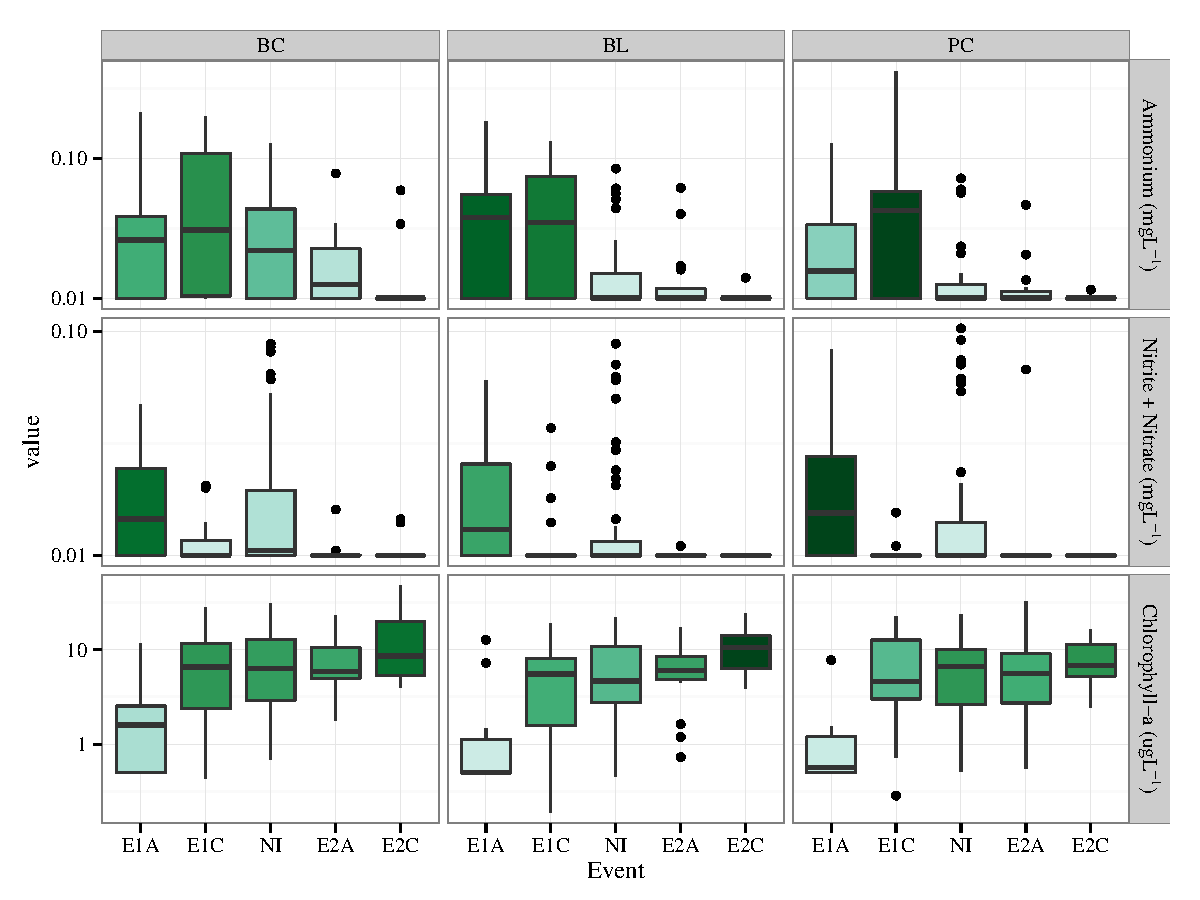
\includegraphics[width=\maxwidth]{figs/boxplt_all-1} 

}

\caption[Boxplot summaries by event of nutrient data at Bayou Cumbest (BC), Bangs Lake (BL), and Point aux Chenes (PC) sites at Grand Bay]{Boxplot summaries by event of nutrient data at Bayou Cumbest (BC), Bangs Lake (BL), and Point aux Chenes (PC) sites at Grand Bay.  Letters indicate significantly different events based on Tukey multiple comparison analyses for each unique site and nutrient value combination.  Boxes represent the interquartile range (IQR, 25\textsuperscript{th} to 75\textsuperscript{th} percentile) with the median as the middle horizonal line.  Boxes are colored by relative median nutrients between sites.  Outliers are present beyond whiskers (1.5$\cdot$IQR). E1A: event 1 acute, E1C: event 1 chronic, NI: non-impact, E2A: event 2 acute, E2C: event 2 chronic.}\label{fig:boxplt_all}
\end{figure}



\end{document}
